\section{Program and Design}  

%%%%%%%%%%%%%%%%%%%%%%%%%%%%%%%%%%%%%%%%%%%%%%%%%%%%%%%%%%%%%%%%%%
%%%%%%%%			OBJECTIVES METHODOLOGY AND RESEARCH
%%%%%%%%%%%%%%%%%%%%%%%%%%%%%%%%%%%%%%%%%%%%%%%%%%%%%%%%%%%%%%%%%%

\subsection{Objectives}

\paragraph{}
The objective of this research project is to attempt to answer the overall question of whether a low voltage DC power distribution system could be implemented to power low load devices such as lighting, simple electronics and charging devices. Secondly, it must be determined whether this is a more efficient solution than existing AC installations. The final objective is to relate this project directly to renewable energy generation and a commercial setting.

\subsection{Methodology}

\paragraph{}
In order to complete this task within a timely manner and ensure all aspects are thoroughly considered and discussed, a clear guideline of tasks musts be followed. Additionally, these tasks will need to specifically address the objectives that the research proposal addresses. As will be further discussed in Section 3, there are five broad questions that are being addressed throughout the two semesters of this thesis. The methodology of the thesis is predominately theoretical and simulation based with the possibility of some physical testing if time permits. A reliance on previous research and design recommendations will be important \cite{Amin2011}. Although research into improving DC systems has increased, this project will be focusing on an area that has not been sufficiently researched and analysed \cite{Pellis1997}.   

\paragraph{}
The five separate questions are related to the same solution. Initial stages of the project require extensive research on the possibilities and theories behind a purely DC system. Once a strong idea of the possibilities and previous papers were analysed a general analysis of whether or not 48 V DC is the ideal voltage level is secondary. To do this, it will be predominately theoretical with voltage drop calculations over standard cable lengths and areas. Additionally research will be used to back up findings. Software and research will be used to assess the options with solar panels and the best method of implementing them into the solution. Queensland University of Technology's Building Management Services provided access to power production and consumption data with both historical and current graphs. Additionally, schematics and floor plans for P and Y Blocks have been given which will assist in the creation of an approximate floor plan for modelling and feasibility. studies.   

\paragraph{}
SMART goals will be used to measure the progress. This framework is based off having goals that are specific, measurable, attainable, realistic and timely. These goals are the milestones that are described. By doing so, tasks can be achieved and a regular logbook of activities maintained for process improvements. Spreadsheets and in-built software data storage will be used to record the findings. These findings will be analysed either through additional hand calculations or Matlab. Figure \ref{fig:PracProcedure} below shows the methodology behind technical design tasks.    

\begin{figure}[H]
\hfill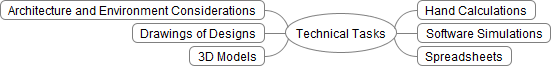
\includegraphics[width = 160mm]{images/Practical_Planning_Rev2}\hspace*{\fill}
\caption{Considerations for a Technical Design Task}
\label{fig:PracProcedure}
\end{figure}     

\newpage

\subsection{Research Plan}

\paragraph{}
A majority of the project will completed through simulations and calculations utilising Dialux4.12, AutoCAD, Microsoft Excel and System Model Advisor. This is due to power systems electronics being expensive and large scale testing out of the financial scope of this project. Ideally, a full system would be built with Photovoltaic cells, battery, controller, DC-DC converters and connections to appliances, however finances will not allow this. Figure \ref{fig:DCHomeSystem} below shows a basic PV DC system and the areas requiring consideration. 

\begin{figure}[H]
\hfill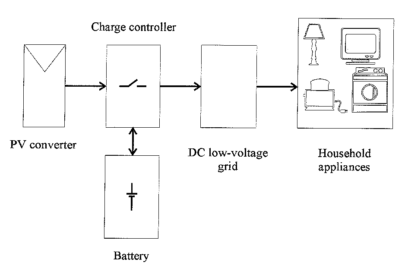
\includegraphics[width = 120mm]{images/DC_Home}\hspace*{\fill}
\caption{Initial Design Consideration for DC Home Power System \cite{Pellis1997}} 
\label{fig:DCHomeSystem}
\end{figure} 

\paragraph{} 
The software will allow for data collection and spreadsheets used to track and assess. The benefit of using spreadsheets and Matlab is that formulas can be input and optimisation simulations run. If simulations are not being used and physical tests are required, a multimeter or computer interfaces will be utilised. If testing cannot be performed or simulated, additional research will be completed to find the closest solution possible. If this method needs to be done, it will explicitly stated in the final report that not all aspects could be physically tested.     

\newpage
%%%%%%%%%%%%%%%%%%%%%%%%%%%%%%%%%%%%%%%%%%%%%%%%%%%%%%%%%%%%%%%%%%
%%%%%%%%			FINANCE
%%%%%%%%%%%%%%%%%%%%%%%%%%%%%%%%%%%%%%%%%%%%%%%%%%%%%%%%%%%%%%%%%%

\subsection{Resources and Funding}

\paragraph{}
The design and construction of this project would require a substantial amount of resources. Due to this, computer assisted design (CAD) programs will be used as the main design calculation feasibility analysis mechanism. The University facilitating this research project will allocate \$50 for each student through purchase order applications. This value will be taken into consideration when designing possible testing mechanisms or models for the presentation. It is unlikely that anything other than computer simulations and rendered images will be used to compliment calculations in the presentation.  

%%%%%%%%%%%%%%%%%%%%%%%%%%%%%%%%%%%%%%%%%%%%%%%%%%%%%%%%%%%%%%%%%%
%%%%%%%%			TEAM
%%%%%%%%%%%%%%%%%%%%%%%%%%%%%%%%%%%%%%%%%%%%%%%%%%%%%%%%%%%%%%%%%%

\subsection{Project Team}

\paragraph{}
As previously stated, this project is being solely undertaken. Although this is the case, there are three undergraduate engineers undertaking topics that are interrelated. In addition to the task discussed within this project report focusing on low voltage DC systems in larger applications, the other two undergraduates are analysing sub-issues in the same broad topic of DC electricity. There will be discussions between the three undergraduates on relevant articles, journals and standards that each individual finds.


%%%%%%%%%%%%%%%%%%%%%%%%%%%%%%%%%%%%%%%%%%%%%%%%%%%%%%%%%%%%%%%%%%
%%%%%%%%			PROGRESS AND REMAINING TASKS
%%%%%%%%%%%%%%%%%%%%%%%%%%%%%%%%%%%%%%%%%%%%%%%%%%%%%%%%%%%%%%%%%%

\subsection{Progress and Remaining Tasks}

\paragraph{}
Appendix item \ref{appendix:Timeline} shows a more detailed and up to date set of timelines with milestones and the dates they were reached or plan to be reached. This section will be a brief description of progress made to this point including specific additions in the most recent 6 months. 

\subsubsection{Completed}

\paragraph{}
The project has progressed into its final stages with the majority of initial analysis having been completed. Sufficient background research and literature review has been completed and the knowledge and information gained from this utilised to complete the report. Skills with the chosen software have been improved in order to effectively model and comment on data. The feedback from the project supervisor has been implemented throughout as it was received. Due to the extensive research, data analysis and draft modelling, the final design phase of the project should progress without delays or failures. 

\subsubsection{Discussion}

\paragraph{}
In the previously mentioned Appendix \ref{appendix:Timeline} it is outlined where siginficant delays were faced. Specifically, further technical calculations and design simulations were completed past pre-planned deadlines. Time was allocated during the summer break for further technical calculations but due to personal travel and commencing full time work immediately upon returning this deadline moved forward. Additionally, meeting and receiving feedback became far more complicated with conflicting schedules. Finally, the initial financial calculations have not been completed due to prioritising design over those calculations. There is no doubt that the finance will be simple to complete once design is finalised. 

\subsubsection{Remaining Tasks} \label{section:remaining-tasks}

\paragraph{}
Throughout the report, there are sections that remain incomplete with notes suggested specifying the intended blank space. Although this documentation process appears incomplete it is to outline more specifically intended discussion and calculation points for the remainder of the project. The final tasks remaining are all part of the final design phase.

\begin{itemize}
	\item Design
	\begin{itemize}
		\item Complete custom design of Brisbane corporate building
		\item Commercial building max demand calculations
		\item Commercial building cable length and voltage drop table
		\item Quantity of photovoltaic modules required
		\item Roof area required to install required modules
		\item Detailed consumption vs production analysis to determine storage or supplementary power requirements
		\item Efficiency comparison
	\end{itemize}

	\item Finance
	\begin{itemize}
		\item Capital investment
		\item Lighting upgrades
		\item Energy savings
		\item Return on investment
		\item Payback period
	\end{itemize}

	\item Documentation
	\begin{itemize}
		\item Tabulate necessary data
		\item Re-work document for flow and remove redundant sections or information
		\item Ensure all acquired data is organised in the appendix
	\end{itemize}

	\item Additional (time permitting)
	\begin{itemize}
		\item Brief room layout for apartment complex
		\item Proposed design for DC distribution in apartment complex
		\item Similar design methodology to the list above
	\end{itemize}
\end{itemize}        
  
